\documentclass[12pt, a4paper]{article}

% --- Essential Packages ---
\usepackage[utf8]{inputenc}
\usepackage[margin=1in]{geometry}
\usepackage{titlesec}
\usepackage{xcolor}
\usepackage{tabularx}
\usepackage{booktabs}
\usepackage{enumitem}
\usepackage{amssymb}
\usepackage{tikz}
\usetikzlibrary{shapes.geometric, arrows.meta, positioning, calc, fit}
\usepackage[most]{tcolorbox}
\usepackage{fancyhdr}
\usepackage[hidelinks]{hyperref}
\usepackage{setspace}

% --- Color Palette (Professional Academic Theme) ---
\definecolor{primary}{RGB}{20, 50, 95}       % Deep Academic Blue
\definecolor{secondary}{RGB}{40, 100, 160}   % Steel Blue
\definecolor{darktext}{RGB}{30, 30, 30}      % Soft Black
\definecolor{lightgray}{RGB}{245, 247, 250}  % Card Background
\definecolor{bordergray}{RGB}{210, 215, 225} % Subtle Border

% --- Spacing & Line Height ---
\setstretch{1.15}
\setlength{\parskip}{0.45em}
\setlength{\parindent}{0pt}

% --- Section Heading Formatting (Prevents word stretching) ---
\titleformat{\section}
  {\raggedright\Large\bfseries\color{primary}}
  {\thesection.}{0.6em}{}
  [\vspace{-0.3em}\color{secondary}\rule{\textwidth}{1pt}\vspace{-0.2em}]

\titleformat{\subsection}
  {\raggedright\large\bfseries\color{secondary}}
  {\thesubsection}{0.5em}{}

\titleformat{\subsubsection}
  {\raggedright\normalsize\bfseries\color{primary}}
  {\thesubsubsection}{0.5em}{}

% --- Running Header & Footer ---
\pagestyle{fancy}
\fancyhf{}
\renewcommand{\headrulewidth}{0.4pt}
\renewcommand{\footrulewidth}{0.4pt}
\fancyhead[L]{\small\color{gray}Project ID: P\_204 \textbar\ Software Requirements Specification (SRS)}
\fancyhead[R]{\small\color{gray}Aptly.AI}
\fancyfoot[C]{\thepage}

\begin{document}

% ==========================================
% 1. COVER PAGE (Official University Design)
% ==========================================
\begin{titlepage}
    % --- Official University Double Border Frame ---
    \begin{tikzpicture}[remember picture, overlay]
        \draw[primary, line width=2pt] 
            ([xshift=13mm, yshift=-13mm]current page.north west) 
            rectangle 
            ([xshift=-13mm, yshift=13mm]current page.south east);
        \draw[secondary!70, line width=0.8pt] 
            ([xshift=14.5mm, yshift=-14.5mm]current page.north west) 
            rectangle 
            ([xshift=-14.5mm, yshift=14.5mm]current page.south east);
    \end{tikzpicture}

    \centering
    \vspace*{0.3cm}
    
    {\large \textbf{\color{primary} DEPARTMENT OF COMPUTER SCIENCE \& ENGINEERING}}\\[0.15cm]
    {\Large \textbf{ABES ENGINEERING COLLEGE, GHAZIABAD}}\\[0.1cm]
    {\footnotesize \textit{(Affiliated to Dr. A.P.J. Abdul Kalam Technical University, Lucknow)}}\\[0.5cm]
    
    {\color{secondary}\rule{0.85\textwidth}{1.2pt}}\\[0.25cm]
    {\LARGE \textbf{\color{primary} SOFTWARE REQUIREMENTS SPECIFICATION}}\\[0.15cm]
    {\normalsize \textbf{Bachelor of Technology in Computer Science \& Engineering}}\\[0.1cm]
    {\small \textit{(Mini Project, Semester VI -- Academic Session 2026--2027)}}\\[0.25cm]
    {\color{secondary}\rule{0.85\textwidth}{1.2pt}}\\[0.8cm]
    
    {\small \textbf{AN SRS DOCUMENT ON}}\\[0.35cm]
    
    {\huge \bfseries \color{primary} AI-Based Resume Screening and}\\[0.25cm]
    {\huge \bfseries \color{primary} Candidate Shortlisting System}\\[0.45cm]
    
    {\Large \textbf{\color{secondary} [ PROJECT CODE: P\_204 ]}}\\[0.3cm]
    {\normalsize \textit{System Implementation: \textbf{Aptly.AI} -- Semantic Multi-Vector ATS \& Talent Pipeline}}\\[1.2cm]
    
    \vfill
    
    % --- Two-Column Parallel Layout: Student Details & Supervisor Details ---
    \begin{minipage}[t]{0.48\textwidth}
        \flushleft
        {\large \textbf{\color{primary} SUBMITTED BY:}}\\[0.25cm]
        \textbf{\large Ayush Kumar Pandey}\\[0.1cm]
        \textbf{University Roll No.:} 2200320100052\\
        \textbf{Branch:} Computer Science \& Engg.\\
        \textbf{Year / Semester:} 3rd Year / 6th Semester
    \end{minipage}
    \hfill
    \begin{minipage}[t]{0.48\textwidth}
        \flushleft
        {\large \textbf{\color{primary} UNDER THE GUIDANCE OF:}}\\[0.25cm]
        \textbf{\large Dr. / Prof. [Guide Name]}\\[0.1cm]
        Assistant Professor\\
        Department of Computer Science \& Engg.\\
        ABES Engineering College, Ghaziabad
    \end{minipage}
    
    \vfill
    \vspace{0.6cm}
    
    {\small \textbf{DEPARTMENT OF COMPUTER SCIENCE AND ENGINEERING}}\\[0.1cm]
    {\large \textbf{\color{primary} ABES ENGINEERING COLLEGE, GHAZIABAD}}\\[0.1cm]
    {\small NH-09, Lal Kuan, Ghaziabad, Uttar Pradesh -- 201009}\\[0.15cm]
    {\footnotesize Submission Date: October 2026}
    \vspace*{0.2cm}
\end{titlepage}

\newpage

% Set section counter to 1 so that the first section starts at 2 (matching the college template)
\setcounter{section}{1}

% ==========================================
% 2. ABSTRACT
% ==========================================
\section{Abstract}
Technical recruitment in high-velocity software engineering domains suffers from severe inefficiencies driven by legacy keyword-based Applicant Tracking Systems (ATS). Traditional keyword filtering drops highly qualified applicants who express equivalent engineering competencies using diverse technical terminology. 

\textbf{Aptly.AI} is an intelligent, multi-vector resume screening and candidate shortlisting platform designed to replace rigid syntactic matching with generative semantic reasoning. The system is engineered as a responsive Single Page Application using React 18, Vite, and Vanilla CSS, powered by a robust backend architecture utilizing Node.js, Express.js (v5), MongoDB Atlas, and Google Gemini LLMs (\texttt{gemini-3.5-flash}). 

The platform implements in-memory stream buffer parsing of binary PDF resumes, multi-vector semantic scoring across core and adjacent technical proficiencies, transparent diagnostic skill-gap scorecards for job seekers, real-time Job Description (JD) clarity and bias analysis for hiring teams, and an interactive Kanban shortlisting pipeline. The expected outcome is a 4.2$\times$ acceleration in screening turnaround, the elimination of keyword-drop errors, and fair, transparent technical evaluations for both candidates and enterprise recruiters.

% ==========================================
% 3. PROBLEM STATEMENT
% ==========================================
\section{Problem Statement}
Conventional technical hiring pipelines suffer from two opposing failure modes that impair both candidates and talent acquisition teams:
\begin{enumerate}[label=\textbf{\arabic*.}]
    \item \textbf{Syntactic Keyword Blindness and High Rejection Latency:} Legacy ATS software evaluates resumes through deterministic string matching. Candidates possessing substantial experience in equivalent or adjacent technologies (e.g., Fastify vs. Express, Podman vs. Docker, PostgreSQL vs. MySQL) are disqualified without conceptual evaluation. Conversely, manual screening requires 3–5 minutes per resume, creating hiring bottlenecks when handling hundreds of submissions.
    \item \textbf{Black-Box Rejections and Biased Job Listings:} Candidates receive uninformative, automated rejection notices that obscure specific technical deficiencies, eliminating actionable learning opportunities. Simultaneously, recruiters unintentionally publish poorly structured job descriptions containing non-inclusive or hyper-aggressive keywords (e.g., ``coding rockstar'', ``ninja''), which degrades applicant diversity and reduces submission quality.
\end{enumerate}

% ==========================================
% 4. OBJECTIVES
% ==========================================
\section{Objectives}
The primary objectives of the Aptly.AI software engineering project are:
\begin{itemize}[leftmargin=1.5em, itemsep=2pt]
    \item \textbf{Develop a User-Friendly, Role-Based Application:} Create intuitive, separate portals for Job Candidates and Enterprise Recruiters with robust security guards.
    \item \textbf{Automate Binary Resume Ingestion:} Implement stream-based PDF extraction to eliminate manual profile form-filling.
    \item \textbf{Eliminate Keyword Screening Bias:} Develop a multi-vector semantic scoring engine that credits adjacent frameworks and production engineering scale.
    \item \textbf{Store and Manage Hiring Data Efficiently:} Architect normalized, high-performance MongoDB Atlas collections for users, vacancies, applications, and AI evaluations.
    \item \textbf{Enforce Job Description Inclusivity:} Build an active client-side analyzer that audits recruiter job postings for clarity, structural completeness, and gendered/exclusionary phrasing.
    \item \textbf{Generate Actionable Diagnostic Reports:} Deliver granular match percentage scorecards (0--100\%), identified skill gaps, custom interview questions, and Kanban stage filtering.
\end{itemize}

\newpage

% ==========================================
% 5. PROPOSED SOLUTION
% ==========================================
\section{Proposed Solution}
Aptly.AI provides an integrated, dual-sided full-stack recruitment platform engineered to automate resume screening and eliminate black-box rejection cycles.

\subsection{How the System Works}
The system operates as an end-to-end recruitment lifecycle manager:
\begin{enumerate}[label=\textbf{\arabic*.}]
    \item \textbf{Job Posting Creation:} A recruiter authors an engineering vacancy. As text is entered, the client-side \textit{JD Quality Panel} assesses readability, structural clarity, and flags exclusionary terminology in real time.
    \item \textbf{Application Submission:} A candidate discovers the job listing, uploads their binary PDF resume, and submits the application.
    \item \textbf{Stream Ingestion \& Entity Extraction:} The backend receives the binary stream via \texttt{multer} directly in memory, utilizes \texttt{pdf-parse} to extract text, and sanitizes character encodings.
    \item \textbf{Multi-Vector Semantic Reasoning:} The extracted text is evaluated against the target JD using Google Gemini LLM with deterministic JSON output schemas. The model assesses core skills, adjacent technologies, and domain tenure.
    \item \textbf{Persistence \& Dashboard Updates:} Evaluation metrics are persisted in MongoDB Atlas, instantly populating the candidate's diagnostic scorecard and updating the recruiter's auto-ranked Kanban pipeline.
\end{enumerate}

\subsection{Main Features}
\begin{itemize}[leftmargin=1.5em, itemsep=2pt]
    \item \textbf{Multi-Vector Semantic Matcher:} Delivers holistic 0--100\% match scores factoring core and transferable technical capabilities.
    \item \textbf{Candidate Diagnostic Scorecards:} Visually categorizes matched vs. missing competencies and provides personalized technical interview prep questions.
    \item \textbf{Real-Time JD Quality \& Inclusivity Panel:} Automatically calculates JD clarity scores (0--100\%) and highlights exclusionary phrases before publishing.
    \item \textbf{Recruiter ATS Kanban Board:} Interactive pipeline (\textit{Applied $\rightarrow$ Shortlisted $\rightarrow$ Technical Interview $\rightarrow$ Offer}) with score-threshold sliders for instant batch filtering.
    \item \textbf{Embedded Conversational AI Copilot:} A global floating assistant providing context-aware guidance on resume optimization and technical interview prep.
\end{itemize}

\subsection{Target Users and Expected Benefits}
\begin{itemize}[leftmargin=1.5em, itemsep=2pt]
    \item \textbf{Candidates / Job Seekers:} Receive instant, transparent evaluations with clear visibility into skill gaps and relevant interview questions.
    \item \textbf{Recruiters / Talent Teams:} Experience 4.2$\times$ faster applicant shortlisting, zero keyword drop errors, and higher-quality, bias-free job postings.
\end{itemize}

\newpage

% ==========================================
% 6. SCOPE OF THE PROJECT
% ==========================================
\section{Scope of the Project}

\subsection{Implemented Scope (Within 4-Day Project Sprint)}
\begin{itemize}[leftmargin=1.5em, itemsep=2pt]
    \item \textbf{Authentication \& RBAC:} Registration, secure login, password hashing (\texttt{bcryptjs}), and stateless JWT authentication isolating Candidate and Recruiter privileges.
    \item \textbf{Resume Processing:} Multipart binary PDF uploading and stream text parsing via \texttt{pdf-parse} without disk persistence.
    \item \textbf{Semantic Evaluation Engine:} Deep reasoning analysis using Google Gemini LLM with structured JSON output schemas.
    \item \textbf{Recruiter ATS Workflow:} Live JD quality auditing, job creation, and interactive Kanban applicant progression with threshold filtering.
    \item \textbf{Diagnostic Candidate Scorecards:} Visual match breakdowns, gap diagnostics, and interview questions.
    \item \textbf{Embedded AI Chatbot:} Reactive conversational copilot with markdown formatting and ATS domain intelligence.
\end{itemize}

\subsection{Out of Current Scope (Future Enhancements)}
\begin{itemize}[leftmargin=1.5em, itemsep=2pt]
    \item Native mobile applications for iOS and Android (currently fully responsive on mobile web).
    \item Automated asynchronous video/audio screening interviews.
    \item Bi-directional enterprise HRMS/payroll integrations (e.g., Workday, SAP SuccessFactors).
\end{itemize}

% ==========================================
% 7. FUNCTIONAL REQUIREMENTS
% ==========================================
\section{Functional Requirements}
The functional requirements describe the specific capabilities and services delivered by Aptly.AI:

\vspace{0.2cm}
\begin{center}
\renewcommand{\arraystretch}{1.2}
\begin{tabularx}{\textwidth}{l p{4.2cm} X}
\toprule
\textbf{\color{primary}ID} & \textbf{\color{primary}Requirement Name} & \textbf{\color{primary}Description} \\
\midrule
\textbf{FR-01} & User Authentication & The system shall support secure registration and JWT login with Candidate and Recruiter role separation. \\
\textbf{FR-02} & Job Vacancy Management & Recruiters shall be able to create, edit, view, and close job postings with structured skill requirements. \\
\textbf{FR-03} & JD Quality Auditing & The system shall evaluate job description text in real time, computing clarity scores and flagging biased phrases. \\
\textbf{FR-04} & Binary Resume Upload & Candidates shall upload PDF resumes via multipart forms, processed in-memory via stream extraction. \\
\textbf{FR-05} & Semantic AI Evaluation & The system shall evaluate extracted resume content against target JDs, returning a 0--100\% score, matched skills, and gaps. \\
\textbf{FR-06} & Diagnostic Scorecards & Candidates shall view transparent evaluation reports with matched vs. missing skills and tailored interview questions. \\
\textbf{FR-07} & Recruiter Kanban Board & Recruiters shall view candidates auto-ranked by match percentage and transition applicants across pipeline stages. \\
\textbf{FR-08} & Dynamic Score Filtering & Recruiters shall filter applicants using an interactive score threshold slider to isolate high-fit profiles. \\
\textbf{FR-09} & Embedded AI Copilot & Users shall interact with a floating chatbot capable of answering domain, technical, and platform queries. \\
\bottomrule
\end{tabularx}
\end{center}

\newpage

% ==========================================
% 8. NON-FUNCTIONAL REQUIREMENTS
% ==========================================
\section{Non-Functional Requirements}
The non-functional requirements define the quality attributes and constraints of the platform:

\begin{itemize}[leftmargin=1.5em, itemsep=4pt]
    \item \textbf{Performance:}
    \begin{itemize}[leftmargin=1.2em]
        \item In-memory resume text parsing and entity normalization shall execute within $\le 300\text{ ms}$.
        \item Full LLM multi-vector semantic scoring shall return complete structured output within $\le 2.0\text{ seconds}$.
        \item Client-side UI transitions and Kanban state updates shall render at 60 FPS without frame dropping.
    \end{itemize}
    \item \textbf{Security:}
    \begin{itemize}[leftmargin=1.2em]
        \item All passwords shall be salted and hashed using \texttt{bcryptjs} (work factor 10) prior to database persistence.
        \item API endpoints shall be protected by signed JSON Web Tokens (JWT) verified via Express middleware.
        \item HTTP headers shall be hardened using \texttt{helmet}, and sensitive API routes protected against brute-force attacks via \texttt{express-rate-limit}.
    \end{itemize}
    \item \textbf{Usability:}
    \begin{itemize}[leftmargin=1.2em]
        \item The user interface shall employ a clean Paper-Card design system with clear typography and high visual contrast.
        \item Critical recruitment actions (applying, filtering, staging) shall require no more than two user clicks.
    \end{itemize}
    \item \textbf{Reliability:}
    \begin{itemize}[leftmargin=1.2em]
        \item The system shall gracefully handle corrupted, encrypted, or non-textual PDF files by returning explicit validation errors.
        \item The AI Chatbot shall incorporate a dual-engine architecture: falling back to an in-memory knowledge engine if external LLM gateways encounter network timeouts.
    \end{itemize}
    \item \textbf{Compatibility:}
    \begin{itemize}[leftmargin=1.2em]
        \item The frontend Single Page Application shall function seamlessly across modern web browsers (Chrome, Edge, Firefox, Safari).
        \item The application layout shall be fully responsive across mobile, tablet, and desktop viewports.
    \end{itemize}
\end{itemize}

% ==========================================
% 9. TECHNOLOGY STACK
% ==========================================
\section{Technology Stack}
The technologies implemented across the Aptly.AI architecture are outlined below:

\vspace{0.2cm}
\begin{center}
\renewcommand{\arraystretch}{1.2}
\begin{tabularx}{\textwidth}{l p{5.0cm} X}
\toprule
\textbf{\color{primary}Component} & \textbf{\color{primary}Technology} & \textbf{\color{primary}Role in Project} \\
\midrule
\textbf{Frontend} & React 18, Vite, Vanilla CSS & Reactive Single Page Application, client routing, paper-card UI \\
\textbf{Backend} & Node.js (v20+), Express.js (v5) & Asynchronous REST API, middleware, security controllers \\
\textbf{Database} & MongoDB Atlas, Mongoose (v9) & Cloud document store for users, jobs, and evaluations \\
\textbf{Artificial Intelligence} & Google Gemini API (\texttt{@google/genai}) & Semantic resume scoring, structured JSON output, AI Copilot \\
\textbf{File Parsing} & \texttt{pdf-parse}, \texttt{multer} & Binary stream ingestion and raw text extraction in memory \\
\textbf{Security \& Auth} & JWT, \texttt{bcryptjs}, Helmet, Rate-Limit & Token auth, credential encryption, rate limiting \\
\textbf{Development IDE} & VS Code / Google Antigravity & Code authoring, debugging, and terminal automation \\
\textbf{Version Control} & Git, GitHub, Vercel & Source tracking, CI/CD automated cloud deployments \\
\bottomrule
\end{tabularx}
\end{center}

\newpage

% ==========================================
% 10. SYSTEM ARCHITECTURE
% ==========================================
\section{System Architecture}
The system architecture of Aptly.AI follows a modular, client-server decoupled paradigm with dedicated stream processing and AI reasoning micro-pipelines:

\vspace{0.4cm}
\centering
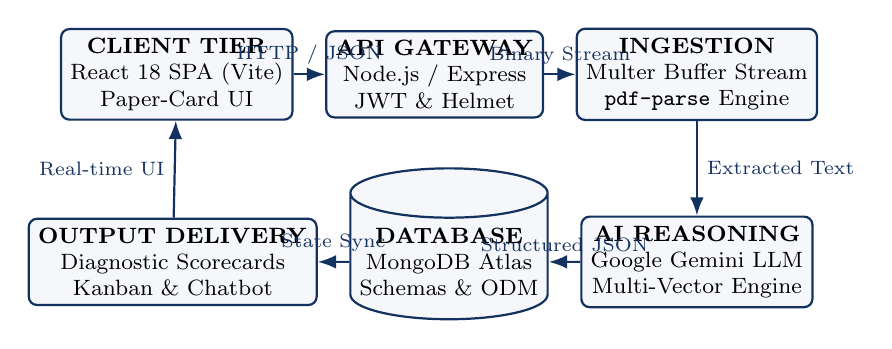
\begin{tikzpicture}[
    node distance=0.7cm and 0.4cm,
    every node/.style={font=\footnotesize},
    layer/.style={rectangle, draw=primary, fill=lightgray, thick, rounded corners=3pt, minimum width=2.6cm, minimum height=0.9cm, align=center},
    db/.style={cylinder, draw=primary, fill=lightgray, shape border rotate=90, aspect=0.25, thick, minimum width=2.4cm, minimum height=1.1cm, align=center},
    arrow/.style={-Latex, thick, primary}
]
    % Nodes
    \node (client) [layer] {\textbf{CLIENT TIER}\\React 18 SPA (Vite)\\Paper-Card UI};
    \node (api) [layer, right=of client] {\textbf{API GATEWAY}\\Node.js / Express\\JWT \& Helmet};
    \node (stream) [layer, right=of api] {\textbf{INGESTION}\\Multer Buffer Stream\\\texttt{pdf-parse} Engine};
    
    \node (ai) [layer, below=1.2cm of stream] {\textbf{AI REASONING}\\Google Gemini LLM\\Multi-Vector Engine};
    \node (db) [db, left=of ai] {\textbf{DATABASE}\\MongoDB Atlas\\Schemas \& ODM};
    \node (output) [layer, left=of db] {\textbf{OUTPUT DELIVERY}\\Diagnostic Scorecards\\Kanban \& Chatbot};

    % Connections
    \draw [arrow] (client) -- node[above]{\scriptsize HTTP / JSON} (api);
    \draw [arrow] (api) -- node[above]{\scriptsize Binary Stream} (stream);
    \draw [arrow] (stream) -- node[right]{\scriptsize Extracted Text} (ai);
    \draw [arrow] (ai) -- node[above]{\scriptsize Structured JSON} (db);
    \draw [arrow] (db) -- node[above]{\scriptsize State Sync} (output);
    \draw [arrow] (output) -- node[left]{\scriptsize Real-time UI} (client);
\end{tikzpicture}
\vspace{0.4cm}

\raggedright
\subsection{Architecture Dataflow Description}
\begin{enumerate}[label=\textbf{\arabic*.}]
    \item \textbf{Presentation Layer (Client Tier):} Built with React 18 and Vite. Houses candidate workflows, recruiter Kanban boards, and the interactive JD quality panel.
    \item \textbf{Application Layer (API Gateway):} Express v5 server enforcing authentication, rate-limiting, CORS, and request routing.
    \item \textbf{Stream Processing Pipeline:} Handles binary resume uploads in memory through \texttt{multer} buffers and converts raw byte streams into sanitized text via \texttt{pdf-parse}.
    \item \textbf{AI Reasoning Layer:} Formulates strict prompt schemas and calls Google Gemini LLM to execute multi-vector semantic distance matching between candidate profiles and job requirements.
    \item \textbf{Persistence Layer:} MongoDB Atlas stores structured documents representing Users, Jobs, and Applications, enabling low-latency queries and real-time dashboard aggregation.
\end{enumerate}

\newpage

% ==========================================
% 11. SYSTEM DESIGN
% ==========================================
\section{System Design}

\subsection{Use Case Diagram}
The Use Case Diagram illustrates the primary actors interacting with Aptly.AI and their functional capabilities:

\vspace{0.3cm}
\centering
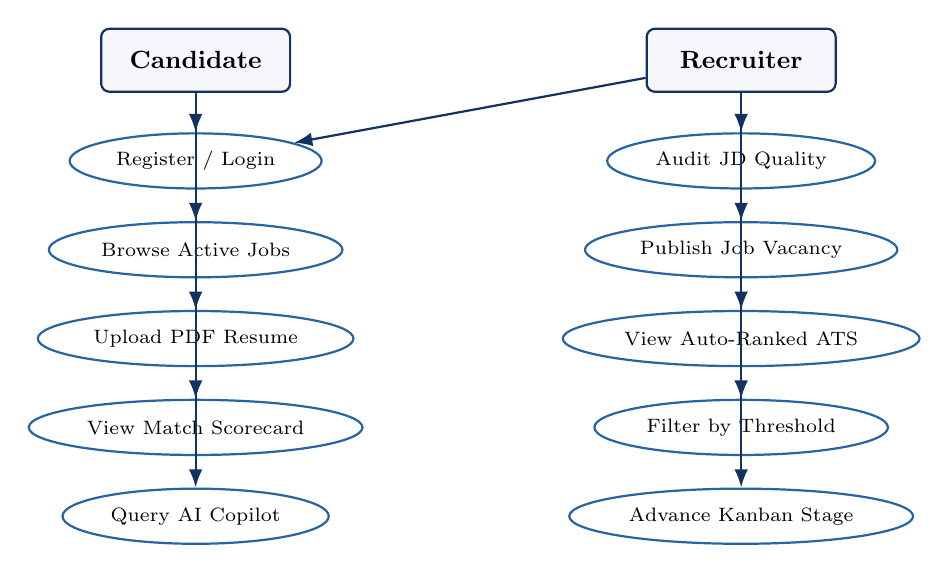
\begin{tikzpicture}[
    node distance=0.6cm and 1.2cm,
    actor/.style={rectangle, draw=primary, fill=lightgray, thick, rounded corners=3pt, minimum width=2.4cm, minimum height=0.8cm, align=center, font=\small\bfseries},
    usecase/.style={ellipse, draw=secondary, fill=white, thick, minimum width=3.2cm, minimum height=0.7cm, align=center, font=\scriptsize},
    arrow/.style={-Latex, thick, primary}
]
    % Actors
    \node (cand) [actor] {Candidate};
    \node (rec) [actor, right=4.5cm of cand] {Recruiter};

    % Candidate Use Cases
    \node (uc1) [usecase, below=0.5cm of cand] {Register / Login};
    \node (uc2) [usecase, below=0.4cm of uc1] {Browse Active Jobs};
    \node (uc3) [usecase, below=0.4cm of uc2] {Upload PDF Resume};
    \node (uc4) [usecase, below=0.4cm of uc3] {View Match Scorecard};
    \node (uc5) [usecase, below=0.4cm of uc4] {Query AI Copilot};

    % Recruiter Use Cases
    \node (uc6) [usecase, below=0.5cm of rec] {Audit JD Quality};
    \node (uc7) [usecase, below=0.4cm of uc6] {Publish Job Vacancy};
    \node (uc8) [usecase, below=0.4cm of uc7] {View Auto-Ranked ATS};
    \node (uc9) [usecase, below=0.4cm of uc8] {Filter by Threshold};
    \node (uc10) [usecase, below=0.4cm of uc9] {Advance Kanban Stage};

    % Connections
    \draw [arrow] (cand) -- (uc1);
    \draw [arrow] (cand) -- (uc2);
    \draw [arrow] (cand) -- (uc3);
    \draw [arrow] (cand) -- (uc4);
    \draw [arrow] (cand) -- (uc5);

    \draw [arrow] (rec) -- (uc1);
    \draw [arrow] (rec) -- (uc6);
    \draw [arrow] (rec) -- (uc7);
    \draw [arrow] (rec) -- (uc8);
    \draw [arrow] (rec) -- (uc9);
    \draw [arrow] (rec) -- (uc10);
\end{tikzpicture}
\vspace{0.4cm}

\raggedright
\subsection{Data Flow Diagram (Level 1 DFD)}
The Level 1 DFD demonstrates the flow of information from resume ingestion to scorecard output:

\vspace{0.3cm}
\centering
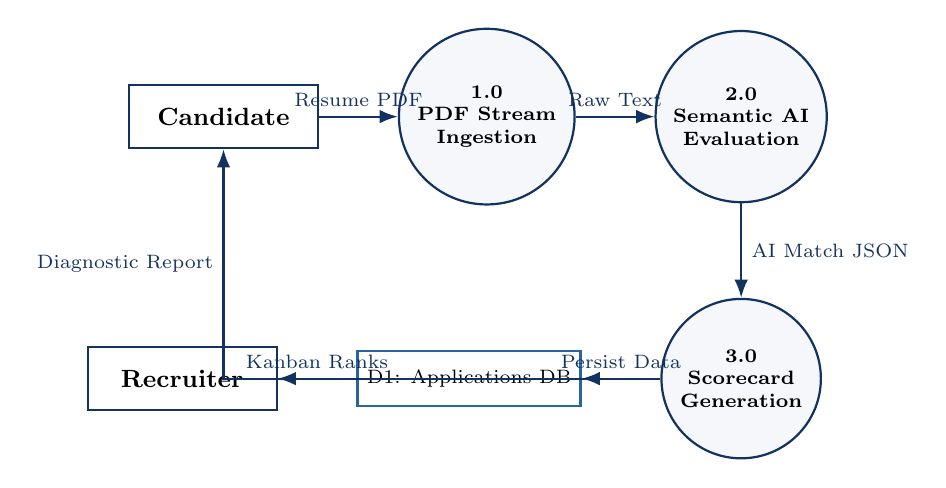
\begin{tikzpicture}[
    node distance=0.8cm and 0.5cm,
    process/.style={circle, draw=primary, fill=lightgray, thick, minimum size=1.8cm, align=center, font=\scriptsize\bfseries},
    entity/.style={rectangle, draw=primary, fill=white, thick, minimum width=2.4cm, minimum height=0.8cm, align=center, font=\small\bfseries},
    store/.style={rectangle, draw=secondary, fill=white, thick, minimum width=2.6cm, minimum height=0.7cm, align=center, font=\scriptsize},
    arrow/.style={-Latex, thick, primary}
]
    \node (user) [entity] {Candidate};
    \node (p1) [process, right=1.0cm of user] {1.0\\PDF Stream\\Ingestion};
    \node (p2) [process, right=1.0cm of p1] {2.0\\Semantic AI\\Evaluation};
    \node (p3) [process, below=1.2cm of p2] {3.0\\Scorecard\\Generation};
    \node (ds) [store, left=1.0cm of p3] {D1: Applications DB};
    \node (rec) [entity, left=1.0cm of ds] {Recruiter};

    \draw [arrow] (user) -- node[above]{\scriptsize Resume PDF} (p1);
    \draw [arrow] (p1) -- node[above]{\scriptsize Raw Text} (p2);
    \draw [arrow] (p2) -- node[right]{\scriptsize AI Match JSON} (p3);
    \draw [arrow] (p3) -- node[above]{\scriptsize Persist Data} (ds);
    \draw [arrow] (ds) -- node[above]{\scriptsize Kanban Ranks} (rec);
    \draw [arrow] (p3) -| node[near end, left]{\scriptsize Diagnostic Report} (user);
\end{tikzpicture}
\vspace{0.3cm}

\newpage

\subsection{Entity-Relationship (ER) Diagram}
The database schema consists of three primary interconnected entities modeled in MongoDB Atlas:

\vspace{0.3cm}
\centering
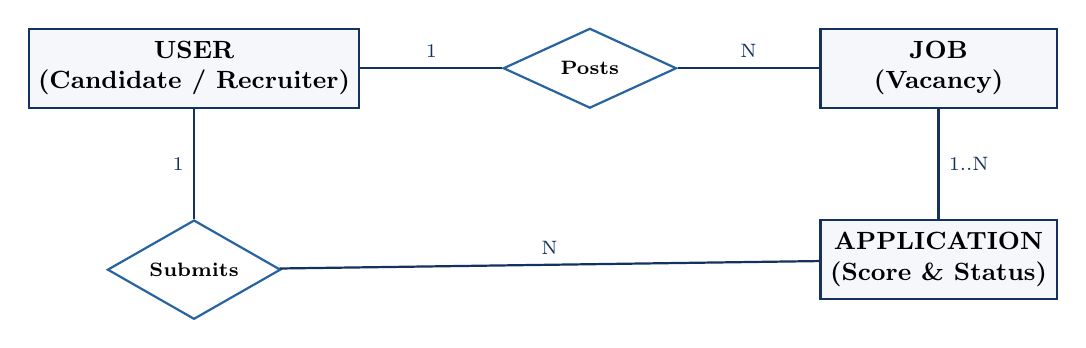
\begin{tikzpicture}[
    node distance=1.2cm and 1.8cm,
    entity/.style={rectangle, draw=primary, fill=lightgray, thick, minimum width=3.0cm, minimum height=1.0cm, align=center, font=\small\bfseries},
    rel/.style={diamond, draw=secondary, fill=white, thick, aspect=1.6, minimum width=2.2cm, minimum height=0.9cm, align=center, font=\scriptsize\bfseries},
    arrow/.style={thick, primary}
]
    \node (user) [entity] {USER\\(Candidate / Recruiter)};
    \node (rel1) [rel, right=of user] {Posts};
    \node (job) [entity, right=of rel1] {JOB\\(Vacancy)};
    \node (rel2) [rel, below=1.4cm of user] {Submits};
    \node (app) [entity, below=1.4cm of job] {APPLICATION\\(Score \& Status)};

    \draw [arrow] (user) -- node[above]{\scriptsize 1} (rel1);
    \draw [arrow] (rel1) -- node[above]{\scriptsize N} (job);
    \draw [arrow] (user) -- node[left]{\scriptsize 1} (rel2);
    \draw [arrow] (rel2) -- node[above]{\scriptsize N} (app);
    \draw [arrow] (job) -- node[right]{\scriptsize 1..N} (app);
\end{tikzpicture}
\vspace{0.4cm}

\raggedright
\subsection{Component and Service Design}
Aptly.AI is structured using the Modular Service-Controller pattern:
\begin{itemize}[leftmargin=1.5em, itemsep=2pt]
    \item \textbf{Client Components:} \texttt{JobCard}, \texttt{ApplyModal}, \texttt{JDQualityPanel}, \texttt{KanbanBoard}, and \texttt{ChatBot}.
    \item \textbf{API Controllers:} \texttt{authController}, \texttt{candidateController}, \texttt{jobController}, and \texttt{chatController}.
    \item \textbf{Core Services:} \texttt{aiEvaluationService} (LLM orchestration) and \texttt{chatService} (hybrid proxy gateway with circuit breaker).
\end{itemize}

% ==========================================
% 12. MODULE DESCRIPTION
% ==========================================
\section{Module Description}
The core operational functionality of Aptly.AI is partitioned into five cohesive modules:

\begin{enumerate}[label=\textbf{Module \arabic* --}, leftmargin=2em, itemsep=5pt]
    \item \textbf{Authentication and Role-Based Access Control (RBAC):}
    \begin{itemize}[leftmargin=1.2em]
        \item Provides registration and login services for Candidates and Recruiters.
        \item Generates cryptographically signed JWT tokens upon credential validation.
        \item Protects private backend endpoints and client routes via \texttt{ProtectedRoute.jsx}.
    \end{itemize}

    \item \textbf{Data Management and Stream-Based Resume Parsing:}
    \begin{itemize}[leftmargin=1.2em]
        \item Ingests multipart binary PDF files directly into memory buffers via \texttt{multer}.
        \item Extracts raw text using \texttt{pdf-parse}, executing whitespace normalization and sanitization.
        \item Prevents filesystem storage overhead and safeguards candidate privacy.
    \end{itemize}

    \item \textbf{Core Processing and Semantic AI Matching Engine:}
    \begin{itemize}[leftmargin=1.2em]
        \item Bridges candidates and job vacancies using Google Gemini LLM reasoning models.
        \item Calculates composite match percentages based on core skills, adjacent frameworks, and tenure.
        \item Returns structured JSON with matched skills, missing skills, and custom interview questions.
    \end{itemize}

    \item \textbf{Job Description Quality and Inclusivity Analyzer:}
    \begin{itemize}[leftmargin=1.2em]
        \item Evaluates recruiter JD text in real time using an active reactive panel.
        \item Computes structural clarity scores and flags gendered or exclusionary buzzwords (e.g., ``rockstar'').
    \end{itemize}

    \item \textbf{Recruiter Kanban Pipeline and Diagnostic Reports:}
    \begin{itemize}[leftmargin=1.2em]
        \item Renders an interactive ATS Kanban board (\textit{Applied $\rightarrow$ Shortlisted $\rightarrow$ Interview $\rightarrow$ Offer}).
        \item Provides real-time score-threshold filtering and generates candidate diagnostic scorecards.
    \end{itemize}
\end{enumerate}

\newpage

% ==========================================
% 13. DATABASE DESIGN
% ==========================================
\section{Database Design}
Aptly.AI utilizes MongoDB Atlas with three primary schemas modeled using Mongoose ODM:

\subsection{Users Collection Schema}
\begin{center}
\renewcommand{\arraystretch}{1.15}
\begin{tabularx}{\textwidth}{l p{3.2cm} X}
\toprule
\textbf{\color{primary}Field Name} & \textbf{\color{primary}Data Type} & \textbf{\color{primary}Description} \\
\midrule
\texttt{\_id} & ObjectId & Unique primary identifier \\
\texttt{name} & String & Full legal name of user \\
\texttt{email} & String (Unique) & User email address (authentication identifier) \\
\texttt{password} & String & Salted bcrypt hash \\
\texttt{role} & String (Enum) & User authorization role: \texttt{'candidate'} or \texttt{'recruiter'} \\
\texttt{skills} & Array of Strings & Self-reported technical skills \\
\texttt{targetRole} & String & Desired candidate job title \\
\texttt{createdAt} & Date & User registration timestamp \\
\bottomrule
\end{tabularx}
\end{center}

\subsection{Jobs Collection Schema}
\begin{center}
\renewcommand{\arraystretch}{1.15}
\begin{tabularx}{\textwidth}{l p{3.2cm} X}
\toprule
\textbf{\color{primary}Field Name} & \textbf{\color{primary}Data Type} & \textbf{\color{primary}Description} \\
\midrule
\texttt{\_id} & ObjectId & Unique job vacancy identifier \\
\texttt{title} & String & Job title (e.g., Full Stack Engineer) \\
\texttt{company} & String & Hiring company name \\
\texttt{description} & String & Full text requirements and role responsibilities \\
\texttt{requiredSkills} & Array of Strings & Key mandatory technical competencies \\
\texttt{postedBy} & ObjectId (Ref: User) & Recruiter who authored the job posting \\
\texttt{createdAt} & Date & Job creation timestamp \\
\bottomrule
\end{tabularx}
\end{center}

\subsection{Applications Collection Schema}
\begin{center}
\renewcommand{\arraystretch}{1.15}
\begin{tabularx}{\textwidth}{l p{3.2cm} X}
\toprule
\textbf{\color{primary}Field Name} & \textbf{\color{primary}Data Type} & \textbf{\color{primary}Description} \\
\midrule
\texttt{\_id} & ObjectId & Unique application submission identifier \\
\texttt{job} & ObjectId (Ref: Job) & Foreign reference to target Job \\
\texttt{candidate} & ObjectId (Ref: User)& Foreign reference to applicant \\
\texttt{resumeUrl} & String & S3/cloud URL or stream reference \\
\texttt{status} & String (Enum) & Pipeline status: \texttt{applied, shortlisted, interview, offer} \\
\texttt{aiMatchScore} & Number (0--100) & Deterministic AI semantic match percentage \\
\texttt{matchedSkills} & Array of Strings & Skills verified in candidate resume \\
\texttt{missingSkills} & Array of Strings & Job requirements absent from resume \\
\texttt{recommendation}& String (Enum) & Category: \texttt{'Strong Match', 'Moderate Match', 'Low Match'} \\
\texttt{appliedAt} & Date & Application submission timestamp \\
\bottomrule
\end{tabularx}
\end{center}

\newpage

% ==========================================
% 14. TESTING
% ==========================================
\section{Testing}
The software platform was validated using functional test cases based on actual implemented modules:

\vspace{0.2cm}
\begin{center}
\renewcommand{\arraystretch}{1.2}
\begin{tabularx}{\textwidth}{l p{3.8cm} p{6.0cm} c}
\toprule
\textbf{\color{primary}Test ID} & \textbf{\color{primary}Test Case} & \textbf{\color{primary}Expected Result} & \textbf{\color{primary}Status} \\
\midrule
\textbf{TC-01} & Valid User Login & Successful JWT issuance and redirect to role dashboard & \textbf{Pass} \\
\textbf{TC-02} & Invalid Password Login & 401 Unauthorized status with descriptive error message & \textbf{Pass} \\
\textbf{TC-03} & In-Memory PDF Upload & Buffer stream extracted into sanitized plain text & \textbf{Pass} \\
\textbf{TC-04} & Multi-Vector Semantic Score & Gemini returns 0--100\% score with matched/missing skills & \textbf{Pass} \\
\textbf{TC-05} & Real-Time JD Quality Check & Clarity score updates dynamically; biased terms flagged & \textbf{Pass} \\
\textbf{TC-06} & Kanban Threshold Filtering & Slider dynamically hides applicants below chosen score & \textbf{Pass} \\
\textbf{TC-07} & Embedded Chatbot Fallback & Returns Gemini response or deterministic knowledge answer & \textbf{Pass} \\
\bottomrule
\end{tabularx}
\end{center}

% ==========================================
% 15. LIMITATIONS
% ==========================================
\section{Limitations}
In accordance with the 4-day mini-project scope, the current system exhibits the following boundaries:
\begin{itemize}[leftmargin=1.5em, itemsep=2.5pt]
    \item \textbf{Rapid Sprint Duration:} Developed and integrated within an intensive 4-day sprint, focusing on core end-to-end user journeys.
    \item \textbf{Text-Based PDF Focus:} Optimal for text-extractable PDFs; scanned graphical image resumes require external OCR preprocessing.
    \item \textbf{No Native Mobile Application:} Currently deployed as a mobile-responsive web app; native iOS/Android packages are not yet published.
    \item \textbf{English Language Optimization:} Semantic taxonomy algorithms and JD bias checks are primarily tuned for English-language resumes.
\end{itemize}

% ==========================================
% 16. FUTURE SCOPE
% ==========================================
\section{Future Scope}
\begin{itemize}[leftmargin=1.5em, itemsep=2.5pt]
    \item \textbf{Cross-Platform Mobile Application:} Package application using React Native with push notifications for application status updates.
    \item \textbf{Cloud Microservices Deployment:} Containerize services with Docker and deploy to Kubernetes for scalable high-load campus recruitment.
    \item \textbf{Automated Video/Audio Screening:} Integrate asynchronous AI voice agents to conduct preliminary technical Q\&A rounds.
    \item \textbf{Advanced Analytics:} Render multi-candidate radar charts comparing depth across technical frameworks.
    \item \textbf{Automated Interview Scheduling:} Integrate Google Calendar and Calendly APIs for instant interview link generation.
\end{itemize}

% ==========================================
% 17. REFERENCES
% ==========================================
\section{References}
\begin{enumerate}[label={[\arabic*]}, leftmargin=2em, itemsep=2.5pt]
    \item Google DeepMind: \textit{Gemini API Structured Outputs and LLM Reasoning Specification}, 2025--2026.
    \item React Team: \textit{React 18 Single Page Application Architecture Guidelines}, 2025.
    \item MongoDB Inc.: \textit{Mongoose Object Data Modeling (ODM) Best Practices}, 2025.
    \item A. Vasiliev et al.: \textit{``Semantic Natural Language Processing in Automated Applicant Tracking Systems,''} IEEE Trans., 2024.
    \item Express.js Team: \textit{Express v5 Routing, Middleware, and Security Architecture}, 2025.
    \item Aptly.AI Live Production Deployment: \url{https://aptly-zeta.vercel.app/}
\end{enumerate}

\vspace{0.3cm}

% ==========================================
% FINAL SRS CHECKLIST
% ==========================================
\subsection*{Final SRS Checklist}
\begin{itemize}[label=$\square$, leftmargin=2em, itemsep=1.5pt]
    \item Cover Page (Official University Frame, Project Code P\_204, Student and Guide Credentials)
    \item Abstract (150--200 words covering project, problem, technologies, outcome)
    \item Problem Statement (Syntactic Keyword Blindness and Lack of Transparency)
    \item Objectives (Six Clear, Measurable Engineering Goals)
    \item Proposed Solution (System Workflow, Features, Users, and Benefits)
    \item Scope of the Project (Implemented Features vs. Out-of-Scope Items)
    \item Functional Requirements (FR-01 to FR-09 Detailed Matrix)
    \item Non-Functional Requirements (Performance, Security, Usability, Reliability, Compatibility)
    \item Technology Stack (Complete Component and Role Matrix)
    \item System Architecture (Detailed TikZ Architecture Pipeline Diagram)
    \item System Design (11.1 Use Case, 11.2 Level-1 DFD, 11.3 ER Diagram, 11.4 Components)
    \item Module Description (Five Core System Modules Defined in Detail)
    \item Database Design (Complete Schemas for User, Job, and Application Collections)
    \item Testing (TC-01 to TC-07 Functional Verification Matrix)
    \item Limitations (Realistic 4-Day Project Scope Boundaries)
    \item Future Scope (Key Planned Advancements)
    \item References (Academic Papers and Official Documentation)
\end{itemize}

\end{document}
